\documentclass{beamer}

\usepackage[T1]{fontenc}
\usepackage{graphicx}
\usepackage{tikz}
\usepackage{booktabs}
\usepackage{minted}
\usepackage{hyperref}
\usepackage[dvipsnames]{xcolor}
\usepackage[spanish]{babel}

\usetikzlibrary{shapes.geometric, arrows.meta, positioning}
\tikzstyle{startstop} = [rectangle, rounded corners, minimum width=3cm, minimum height=1cm,text centered, draw=black, fill=blue!20]
\tikzstyle{process} = [rectangle, minimum width=3.2cm, minimum height=1cm, text centered, draw=black, fill=gray!10]
\tikzstyle{io} = [trapezium, trapezium left angle=70, trapezium right angle=110, minimum width=3.2cm, minimum height=1cm, text centered, draw=black, fill=orange!20]
\tikzstyle{arrow} = [thick, ->, >=stealth]
\usemintedstyle{manni}

\usetheme{Berlin}
\setbeamercolor{structure}{fg=RoyalPurple}

\title[Motor y editor de videojuegos en 2D enfocado al desarrollo de juegos RPG]{Motor y editor de videojuegos en 2D enfocado al desarrollo de juegos RPG}
\subtitle{2D video game engine and editor focused on RPG game development}
\author[Miguel Curros, Alejandro González y Alejandro Massó]{Miguel Curros García\\ Alejandro González Sánchez\\ Alejandro Massó Martínez}
\date{10 de junio de 2025}

\newcommand{\baker}{%
	\textsc{RPGBaker}%
}

\newcommand{\comillas}[1]{\guillemotleft #1\guillemotright{}}

\begin{document}

\frame{\titlepage}

\begin{frame}{Índice}
	\tableofcontents
\end{frame}

\section{Objetivos}
\begin{frame}{Objetivos}
	\begin{columns}
		\column{0.5\textwidth}
		\begin{itemize}
			\item Motor 2D multiplataforma orientado a RPG.
			\item Juegos definidos en archivos de datos.
			\item Editor que permita diseñar los juegos.
		\end{itemize}
		\column{0.5\textwidth}
		
\includegraphics[width=\textwidth]{imgs/objetivos/android.pdf}
	\end{columns}
\end{frame}

\section{Herramientas}
\begin{frame}{Herramientas}
	\begin{columns}
		\column{0.5\textwidth}
		\begin{itemize}
			\item Desarrollo en C++.
			\item Motor con SDL.
			\item Archivos de datos en Lua.
			\item Editor con SDL y DearImGui.
		\end{itemize}
		\column{0.5\textwidth}
		\begin{center}
			
\includegraphics[width=0.6\textwidth]{imgs/herramientas/sdl.pdf}
			\begin{columns}
				\column{0.4\textwidth}
				
\includegraphics[width=\textwidth]{imgs/herramientas/lua.pdf}
				\column{0.6\textwidth}
				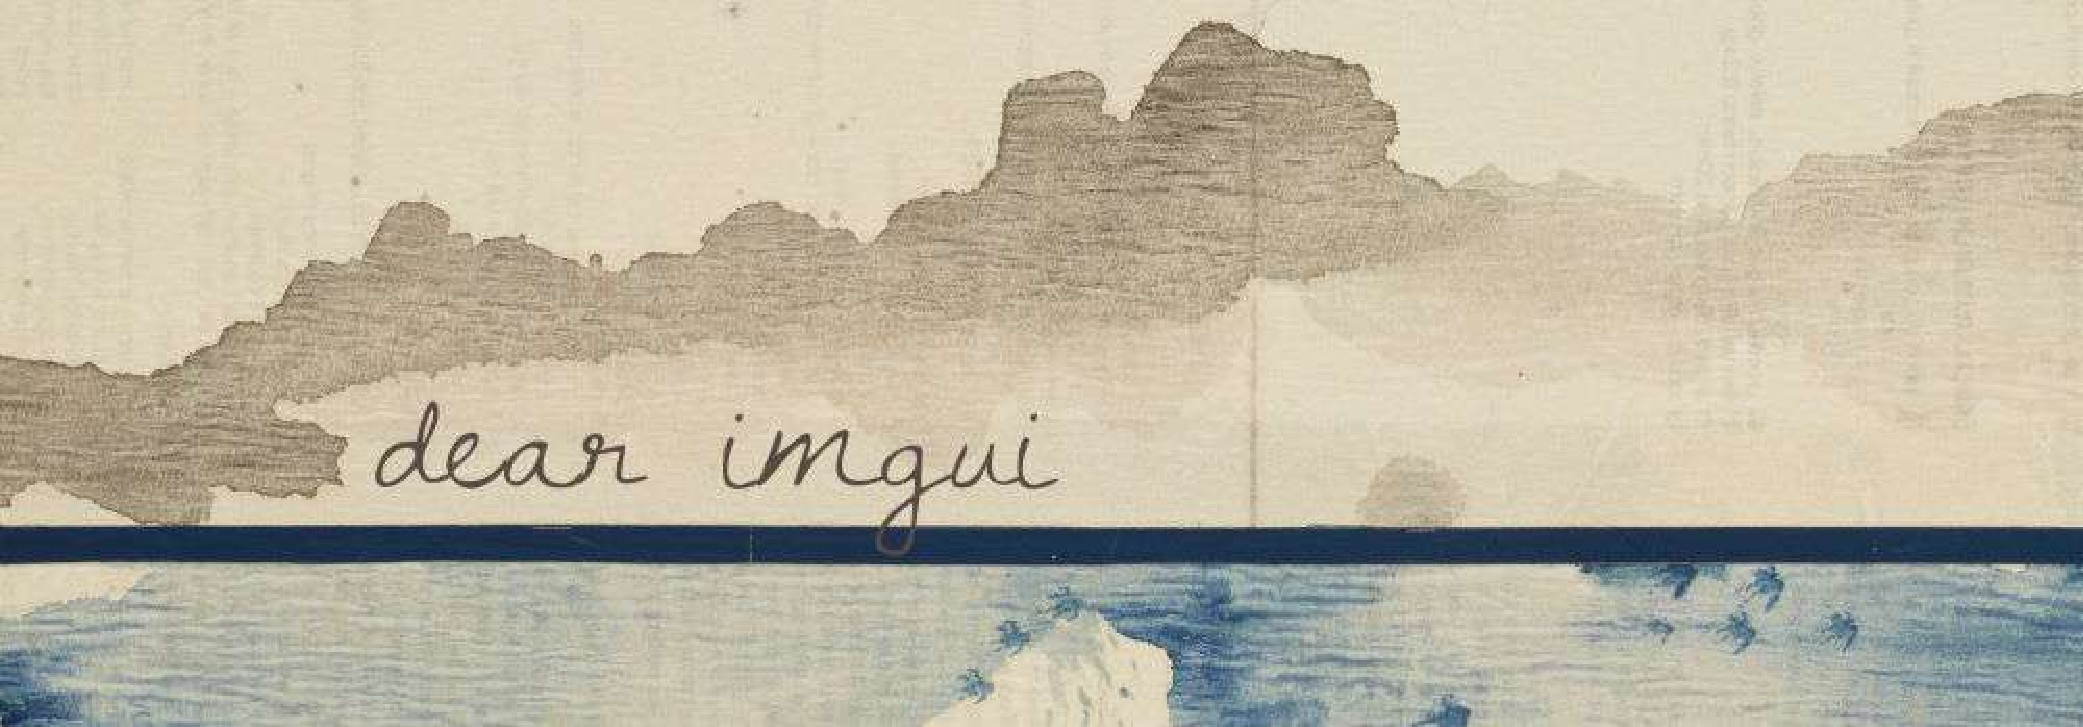
\includegraphics[width=\textwidth]{imgs/herramientas/dearimgui.pdf}
			\end{columns}
		\end{center}
	\end{columns}
\end{frame}
\section{Diseño del motor de \baker}
\begin{frame}{\textit{Core}}
	\begin{columns}
		\column{0.4\textwidth}
			\begin{itemize}
				\item Sistema de entidad componente.
				\item Sistema de recursos.
			\end{itemize}
	 	\column{0.6\textwidth}
			\begin{tikzpicture}
				\begin{class}[text width=5cm]{SceneManager}{-1,0}
					\attribute{- scenes : list<Scene>}
					\operation{+ addScene(string): Scene}
					\operation{+ popScene() : void}
					\operation{+ update() : bool}
					\operation{+ render() : bool}
				\end{class}
				\begin{class}[text width=5cm]{Scene}{7,0}
					\attribute{- entities : list<Entity>}
					\operation{+ init() : bool}
					\operation{+ update() : bool}
					\operation{+ render() : bool}
					\operation{+ refresh() : void}
				\end{class}
				\begin{class}[text width=5cm]{Entity}{7,-5}
					\attribute{- enabled : bool}
					\attribute{- components : list<Component>}
					\operation{+ init() : bool}
					\operation{+ update() : bool}
					\operation{+ fixedUpdate() : bool}
					\operation{+ setEnabled(bool) : bool}
				\end{class}
				\begin{class}[text width=5cm]{Component}{-1,-5}
					\attribute{- enabled : bool}
					\attribute{- entity : Entity}
					\operation{+ init() : bool}
					\operation{+ update() : bool}
					\operation{+ setEnabled(bool) : bool}
					\operation{+ onEnabled() : bool}
					\operation{+ onDisabled() : bool}
				\end{class}
				\composition{SceneManager}{}{}{Scene}
				\aggregation{Scene}{}{}{Entity}
				\composition{Entity}{}{}{Component}
			\end{tikzpicture}
	\end{columns}
\end{frame}
\begin{frame}{Componentes genéricos}
	\begin{columns}
		\column{0.4\textwidth}
			\begin{itemize}
				\item Sistema de \textit{renderizado}.
				\item Sistema de audio.
				\item Sistema de \textit{input}.
				\item Sistema de colisiones.		
			\end{itemize}
	 	\column{0.6\textwidth}
		 	\begin{tikzpicture}[
		 		bigbox/.style={rectangle, draw, thick, minimum width=6cm, minimum height=3cm, fill=#1!20},
		 		subbox/.style={rectangle, draw, thick, minimum width=4.5cm, minimum height=0.8cm, fill=white},
		 		innerbox/.style={rectangle, draw, thick, minimum width=3.5cm, minimum height=0.6cm, fill=white},
		 		node distance=0.6cm,
		 		font=\sffamily
		 		]
		 		% Render
		 		\node[bigbox=blue, label=above:{\textbf{Render}}] (render) at (0,0) {};
		 		\node[subbox] (camera) [below left=0.2cm and 0.3cm of rendercomp.north] {Camera};
		 		\node[subbox] (rectangle) [below=0.2cm of camera] {Rectangle};
		 		\node[subbox] (text) [below=0.2cm of rectangle] {Text};
		 		\node[subbox] (sprite) [right=0.5cm of rectangle] {SpriteRenderer};
		 		\node[innerbox] (animator) [below=0.2cm of sprite] {Animator};
		 		% Audio
		 		\node[bigbox=orange, label=above:{\textbf{Audio}}] (audio) [right=5.5cm of render] {};
		 		\node[subbox] (audiosource) [below left=0.2cm and 0.3cm of audio.north] {AudioSource};
		 		\node[subbox] (audiomixer) [below=0.2cm of audiosource] {AudioMixer};
		 		\node[subbox] (audioclip) [below=0.2cm of audiomixer] {AudioClip};
		 		% Input
		 		\node[bigbox=green, label=above:{\textbf{Input}}] (input) [below=4.5cm of rendercomp.south] {};
		 		\node[subbox] (inputstate) [below left=0.2cm and 0.3cm of input.north] {InputState};
		 		\node[subbox] (button) [below=0.2cm of inputstate] {Button};
		 		% Collisions
		 		\node[bigbox=red, label=above:{\textbf{Collisions}}] (collisions) [right=5.5cm of input] {};
		 		\node[subbox] (collider) [below=0.5cm of collisions.north] {Collider};
		 		% Conexión SpriteRenderer -> Animator
		 		\draw[-{Latex[length=2mm]}, thick] (sprite.south) -- (animator.north);
		 	\end{tikzpicture}
	\end{columns}
\end{frame}
\begin{frame}{Componentes específicos}
	\begin{columns}
		\column{0.4\textwidth}
			\begin{itemize}
				\item Sistema de diálogos.
				\item Sistema de movimiento.
				\item Sistema de mapas.
				\item Sistema de eventos.
			\end{itemize}
	 	\column{0.6\textwidth}
		 	\begin{tikzpicture}[
		 		bigbox/.style={rectangle, draw, thick, minimum width=6cm, minimum height=3cm, fill=#1!20},
		 		subbox/.style={rectangle, draw, thick, minimum width=4.5cm, minimum height=0.8cm, fill=white},
		 		node distance=0.6cm,
		 		font=\sffamily
		 		]
		 		% Dialogue
		 		\node[bigbox=violet, label=above:{\textbf{Dialogue}}] (dialogue) at (0,0) {};
		 		\node[subbox] (textbox) [below left=0.2cm and 0.3cm of dialogue.north] {TextBox};
		 		\node[subbox] (choices) [below=0.2cm of textbox] {Choices};
		 		% Movement
		 		\node[bigbox=cyan, label=above:{\textbf{Movement}}] (movement) [right=6.5cm of dialogue] {};
		 		\node[subbox] (movemgr) [below left=0.2cm and 0.3cm of movement.north] {MovementManager};
		 		\node[subbox] (moveobst) [below=0.2cm of movemgr] {MovementObstacle};
		 		\node[subbox] (movecomp) [below=0.2cm of moveobst] {MovementComponent};
		 		% Maps
		 		\node[bigbox=green, label=above:{\textbf{Maps}}] (maps) [below=4.5cm of dialogue.south] {};
		 		\node[subbox] (overworld) [below left=0.2cm and 0.3cm of maps.north] {OverworldManager};
		 		\node[subbox] (mapcomp) [below=0.2cm of overworld] {MapComponent};
		 		% Events
		 		\node[bigbox=orange, label=above:{\textbf{Events}}] (events) [right=6.5cm of maps] {};
		 		\node[subbox] (eventhandler) [below left=0.2cm and 0.3cm of events.north] {EventHandler};
		 		\node[subbox] (localvars) [below=0.2cm of eventhandler] {LocalVariables};
		 	\end{tikzpicture}
	\end{columns}
\end{frame}
\begin{frame}{Eventos}
	\begin{columns}
		\column{0.4\textwidth}
			\begin{itemize}
				\item \textit{Conditions}.
				\item \textit{Behaviours}.
				\item Integración con el editor.
			\end{itemize}
	 	\column{0.6\textwidth}
	 		\begin{tikzpicture}[every node/.style={font=\small}]
	 			\begin{class}[text width=5cm]{Event}{3,0}
	 				\attribute{- condition : EventCondition}
	 				\attribute{- behaviours : vector<EventBehaviour>}
	 				\operation{+ update() : bool}
	 				\operation{+ start() : void}
	 				\operation{+ resume() : void}
	 				\operation{+ pause() : void}
	 				\operation{+ stop() : void}
	 				\operation{+ jump(int) : void}
	 			\end{class}
	 			\begin{class}[text width=3cm]{EventCondition}{-1,-7}
	 				\attribute{- scene : Scene}
	 				\attribute{- entity : Entity}
	 				\attribute{- event : Event}
	 				\operation{+ met() : bool}
	 			\end{class}
	 			\begin{class}[text width=4cm]{EventBehaviour}{7,-7}
	 				\attribute{- manager : SceneManager}
	 				\attribute{- scene : Scene}
	 				\attribute{- entity : Entity}
	 				\attribute{- event : Event}
	 				\operation{+ init() : bool}
	 				\operation{+ onStart() : bool}
	 				\operation{+ act() : bool}
	 				\operation{+ done() : bool}
	 			\end{class}
	 			\composition{Event}{}{}{EventCondition}
	 			\composition{Event}{}{}{EventBehaviour}
	 		\end{tikzpicture}
	\end{columns}
\end{frame}
\section{Diseño del editor de \baker}
\begin{frame}{Editor de \baker}
	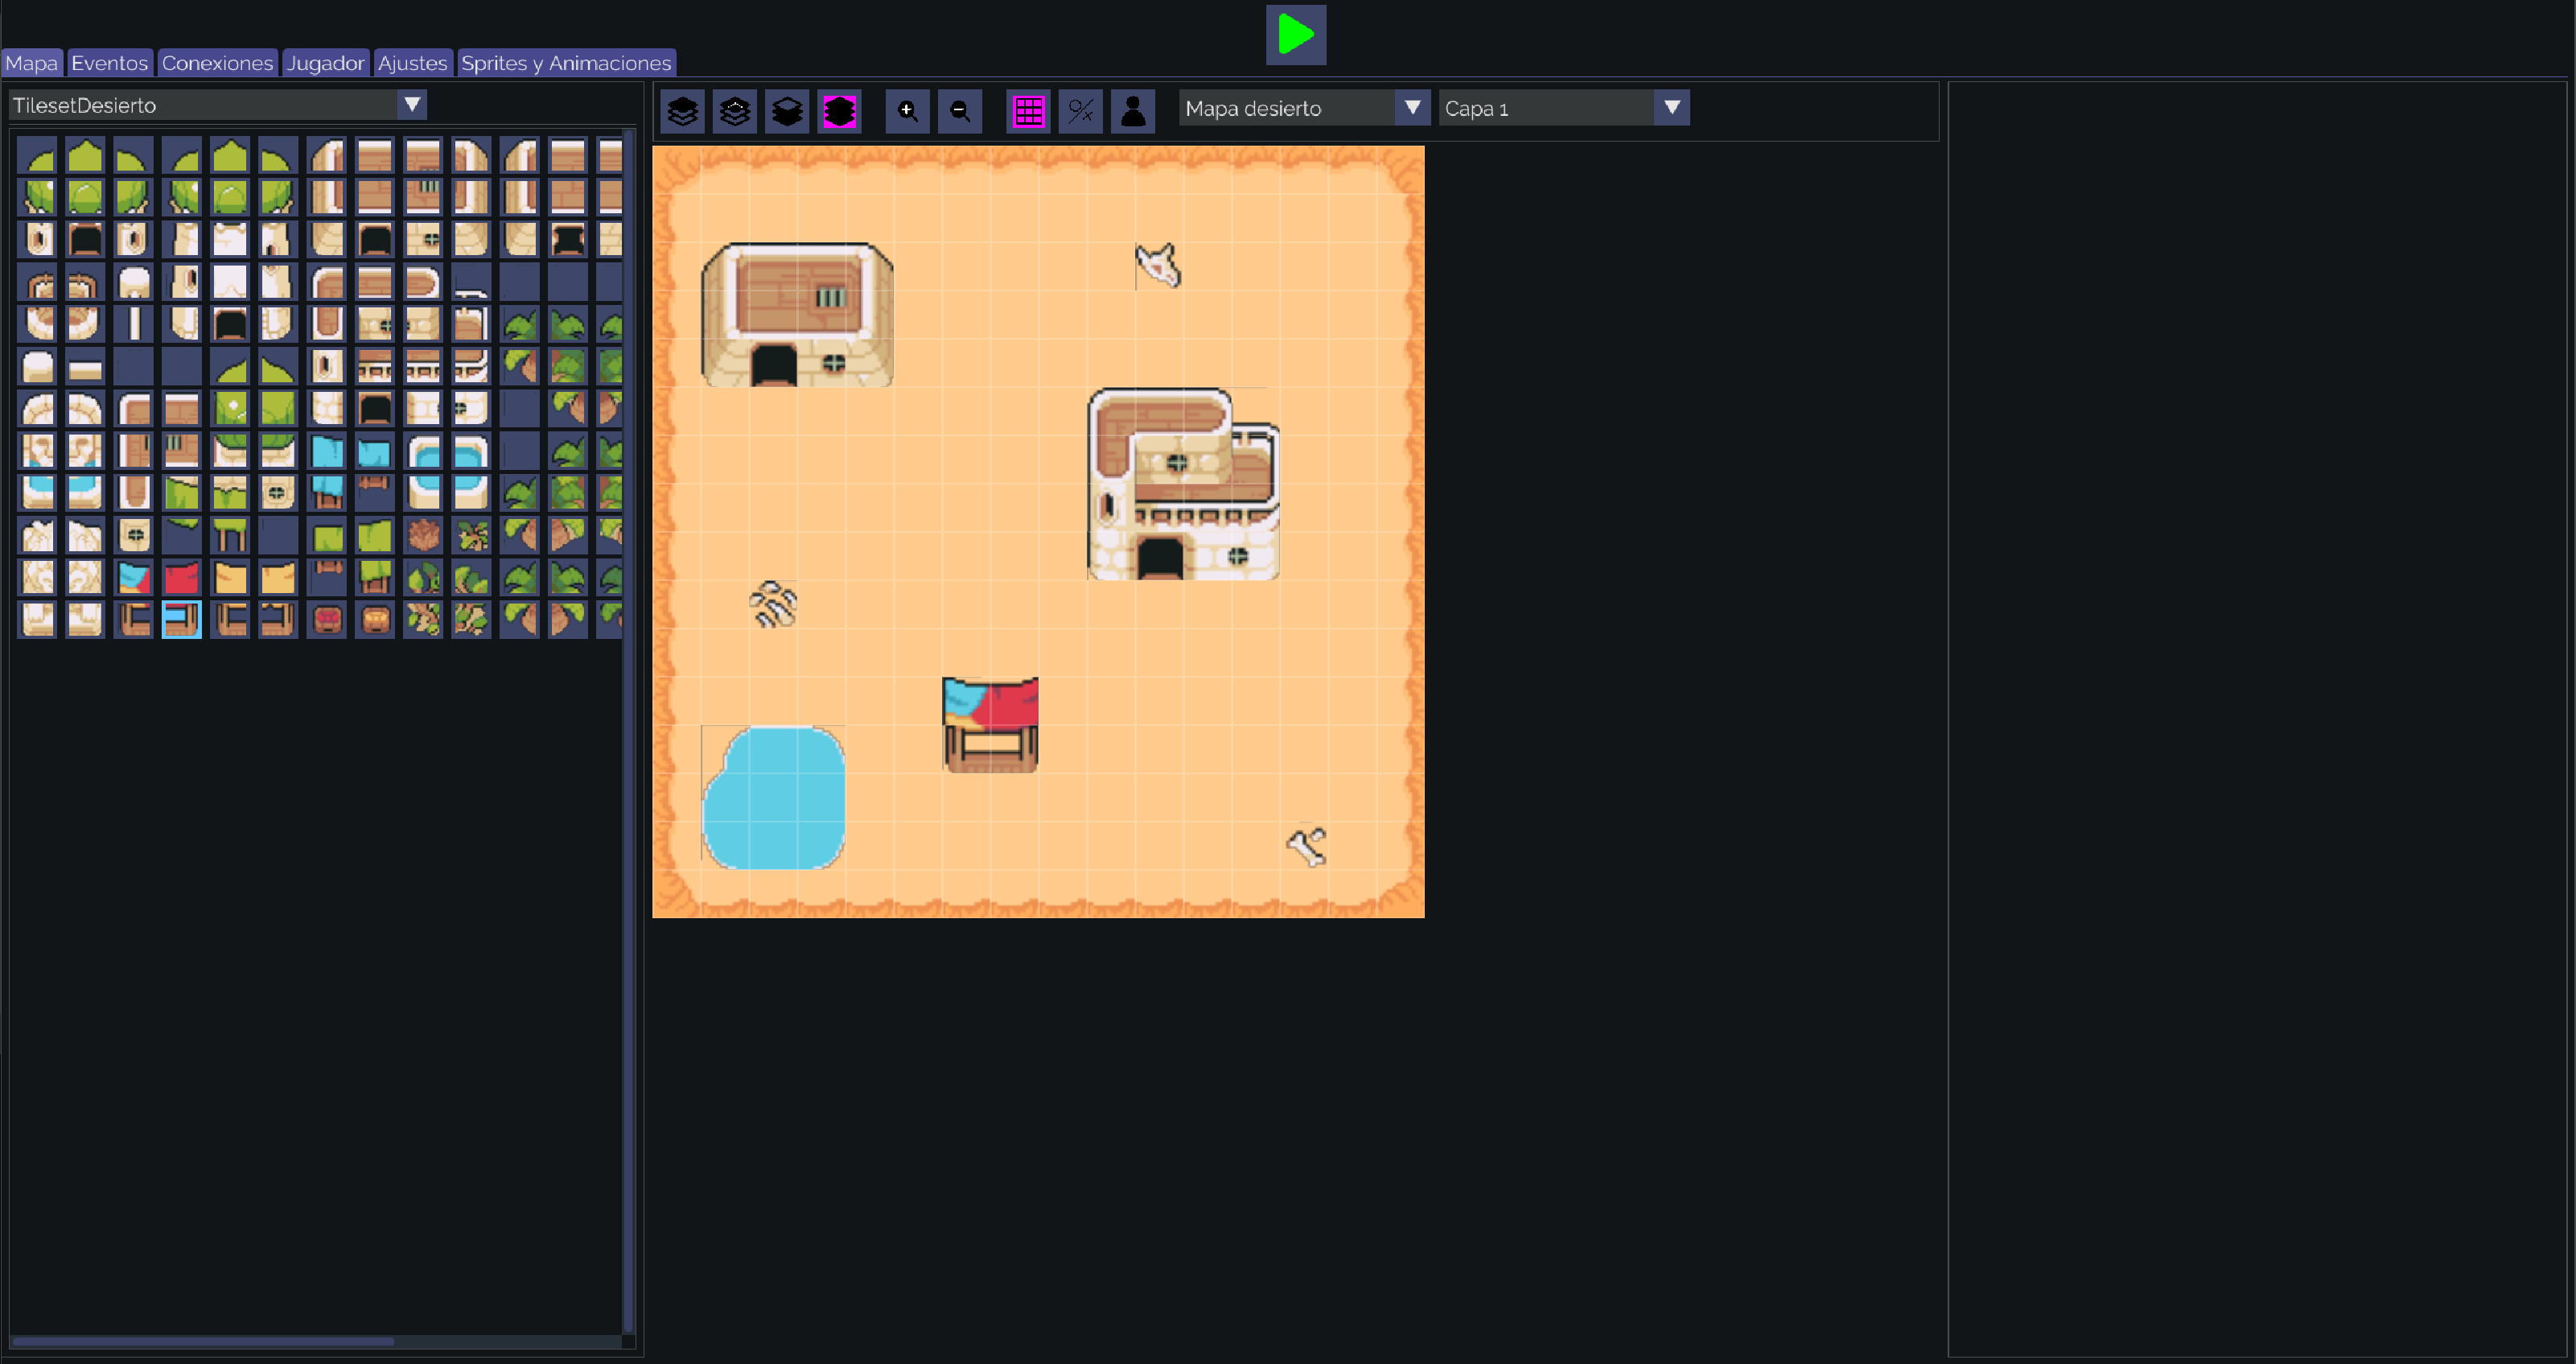
\includegraphics[width=\textwidth]{imgs/editor/editorMapas.pdf}
\end{frame}

\begin{frame}{Funcionalidades principales}
	\begin{columns}
		\column{0.4\textwidth}
			\begin{itemize}
				\item Edición de mapas de manera interactiva.
				\item Gestión de recursos gráficos, como \textit{sprites} o animaciones.
				\item Edición de eventos con condiciones y comportamientos personalizables.
				\item Carga y guardado de proyectos con persistencia completa.
			\end{itemize}
		\column{0.6\textwidth}
			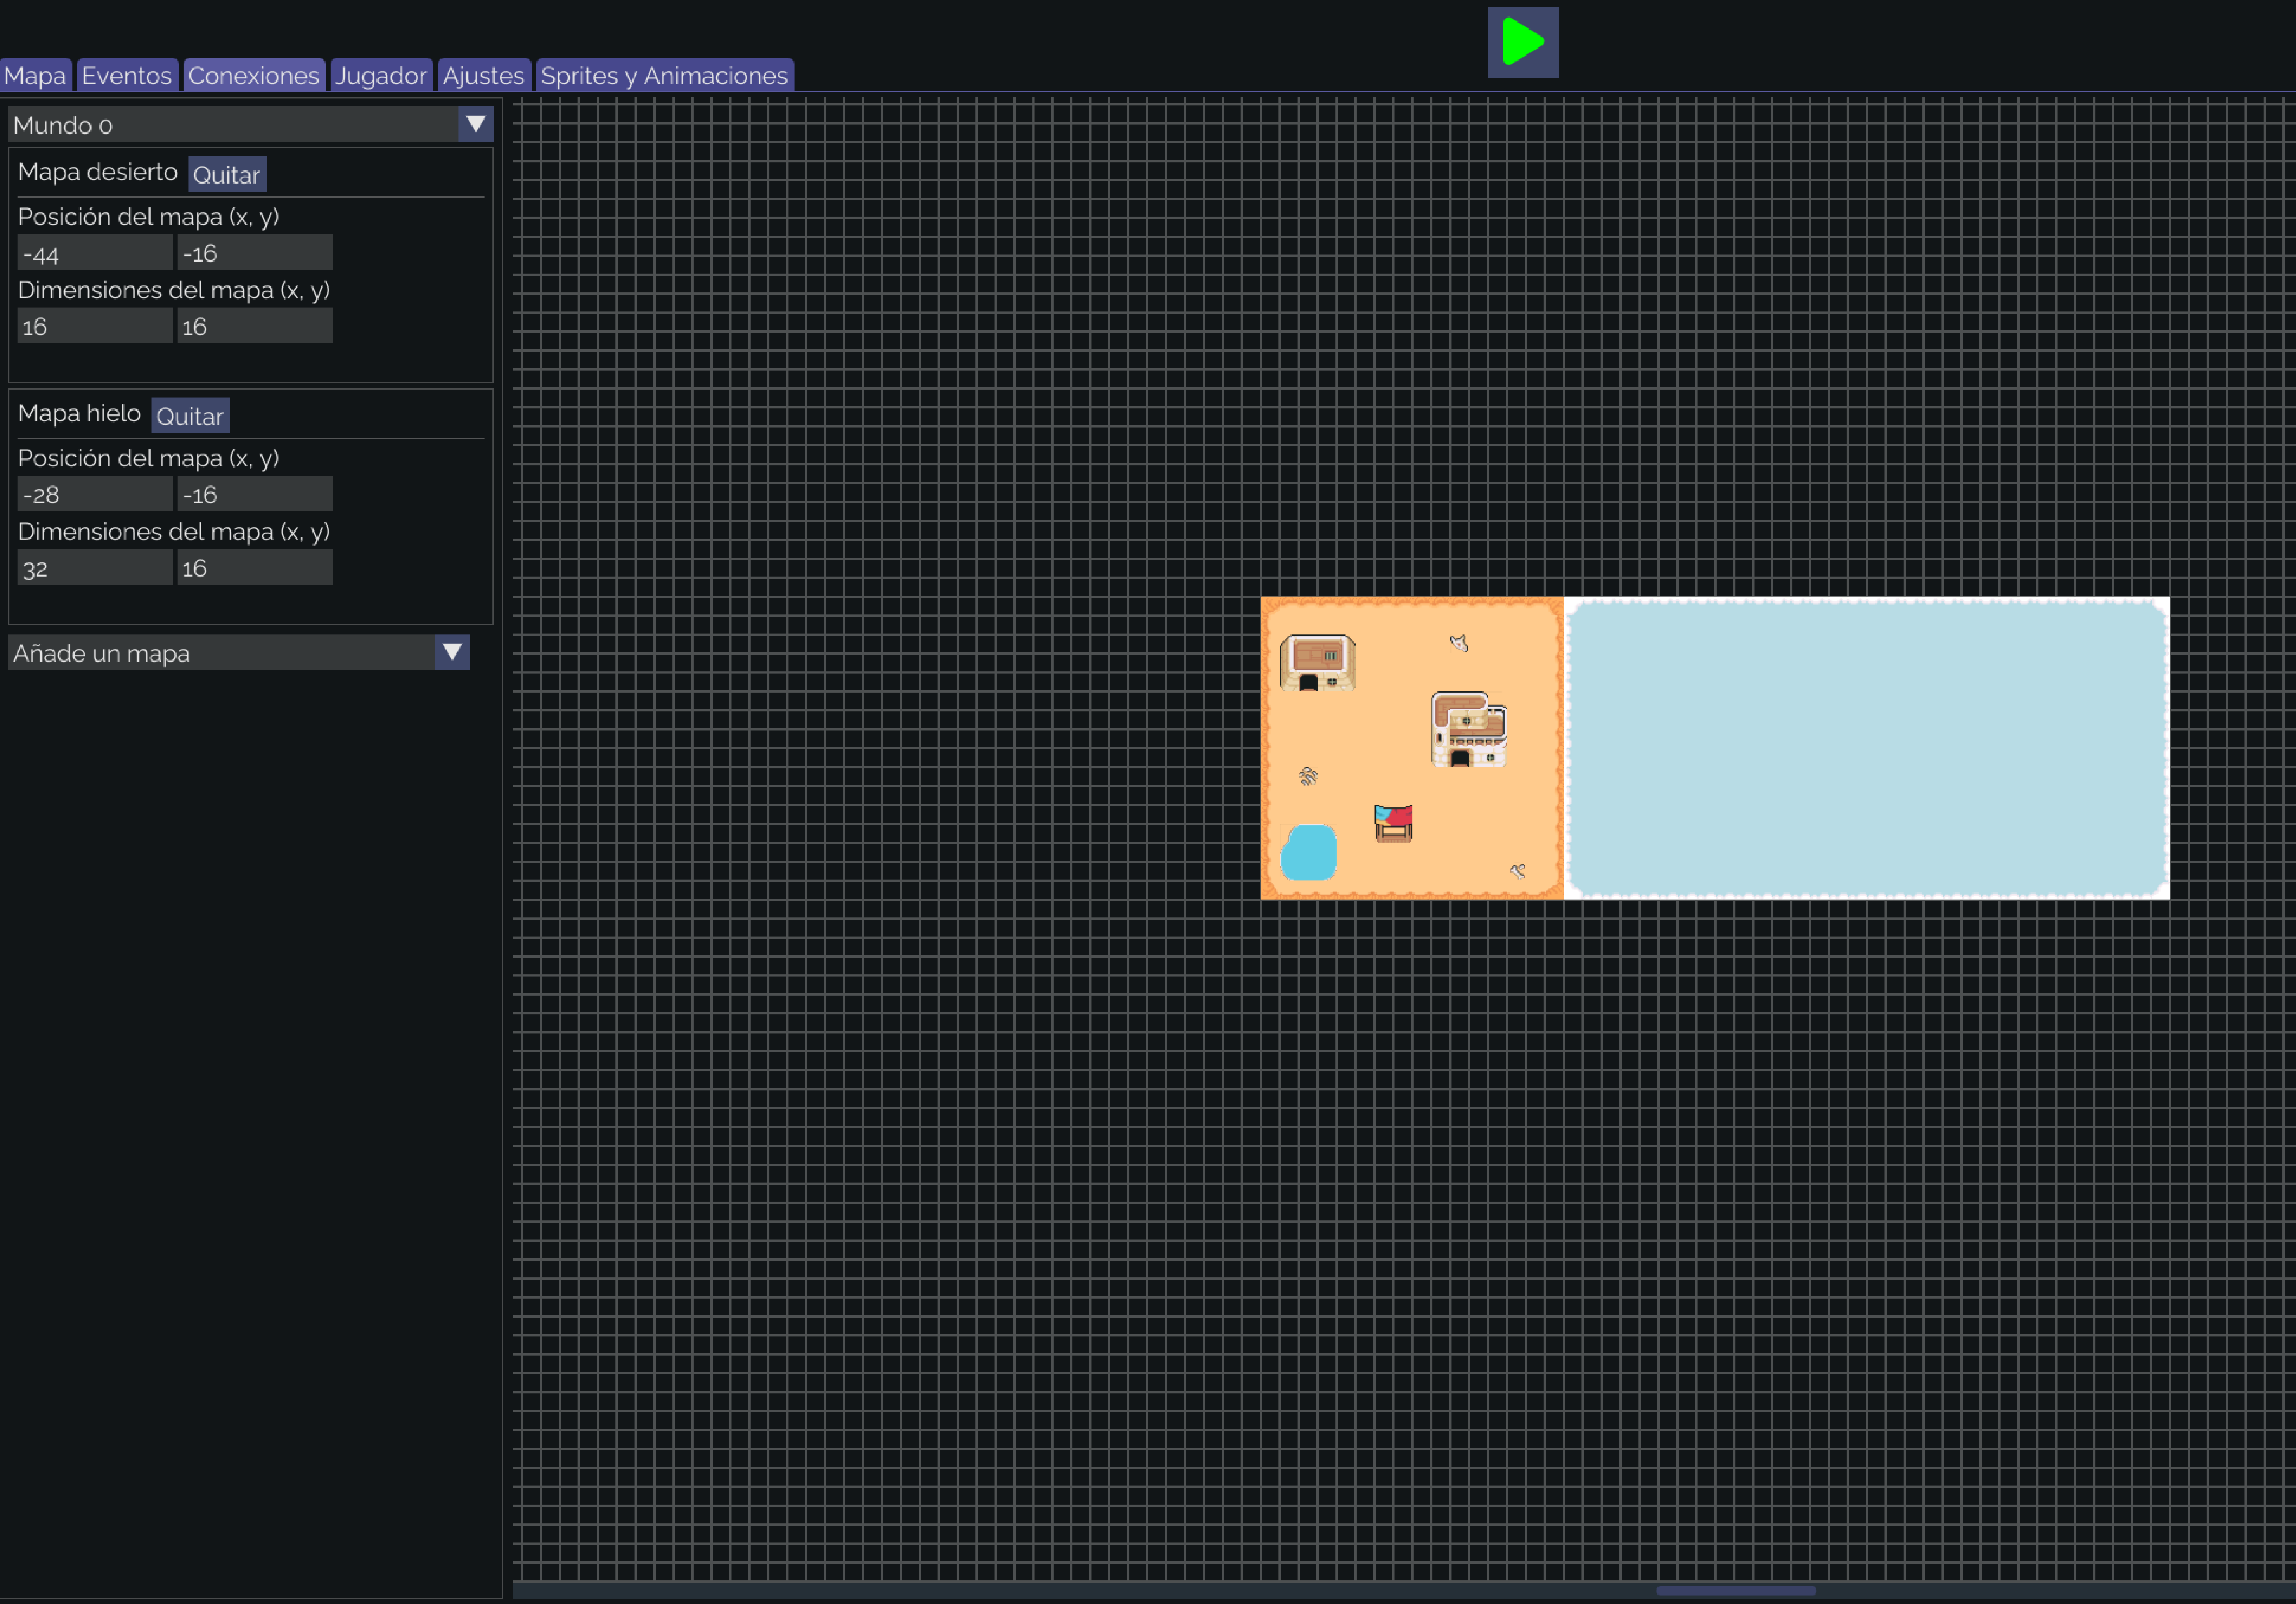
\includegraphics[width=\textwidth]{imgs/editor/conexiones.pdf}
	\end{columns}
\end{frame}

\begin{frame}{Interfaz y usabilidad}
	\begin{columns}
		 \column{0.4\textwidth}
		 	\begin{itemize}
		 		\item Interfaz basada en ventanas y pestañas: clara, modular y adaptable.
		 		\item Pensada para usuarios novatos.
		 		\item Pestañas dependiendo de su función: editor de mapas, de eventos, de recursos\ldots
		 		\item Soporte de elementos visuales como \textit{tooltips} o mensajes de error.
		 	\end{itemize}
		 \column{0.6\textwidth}
		 	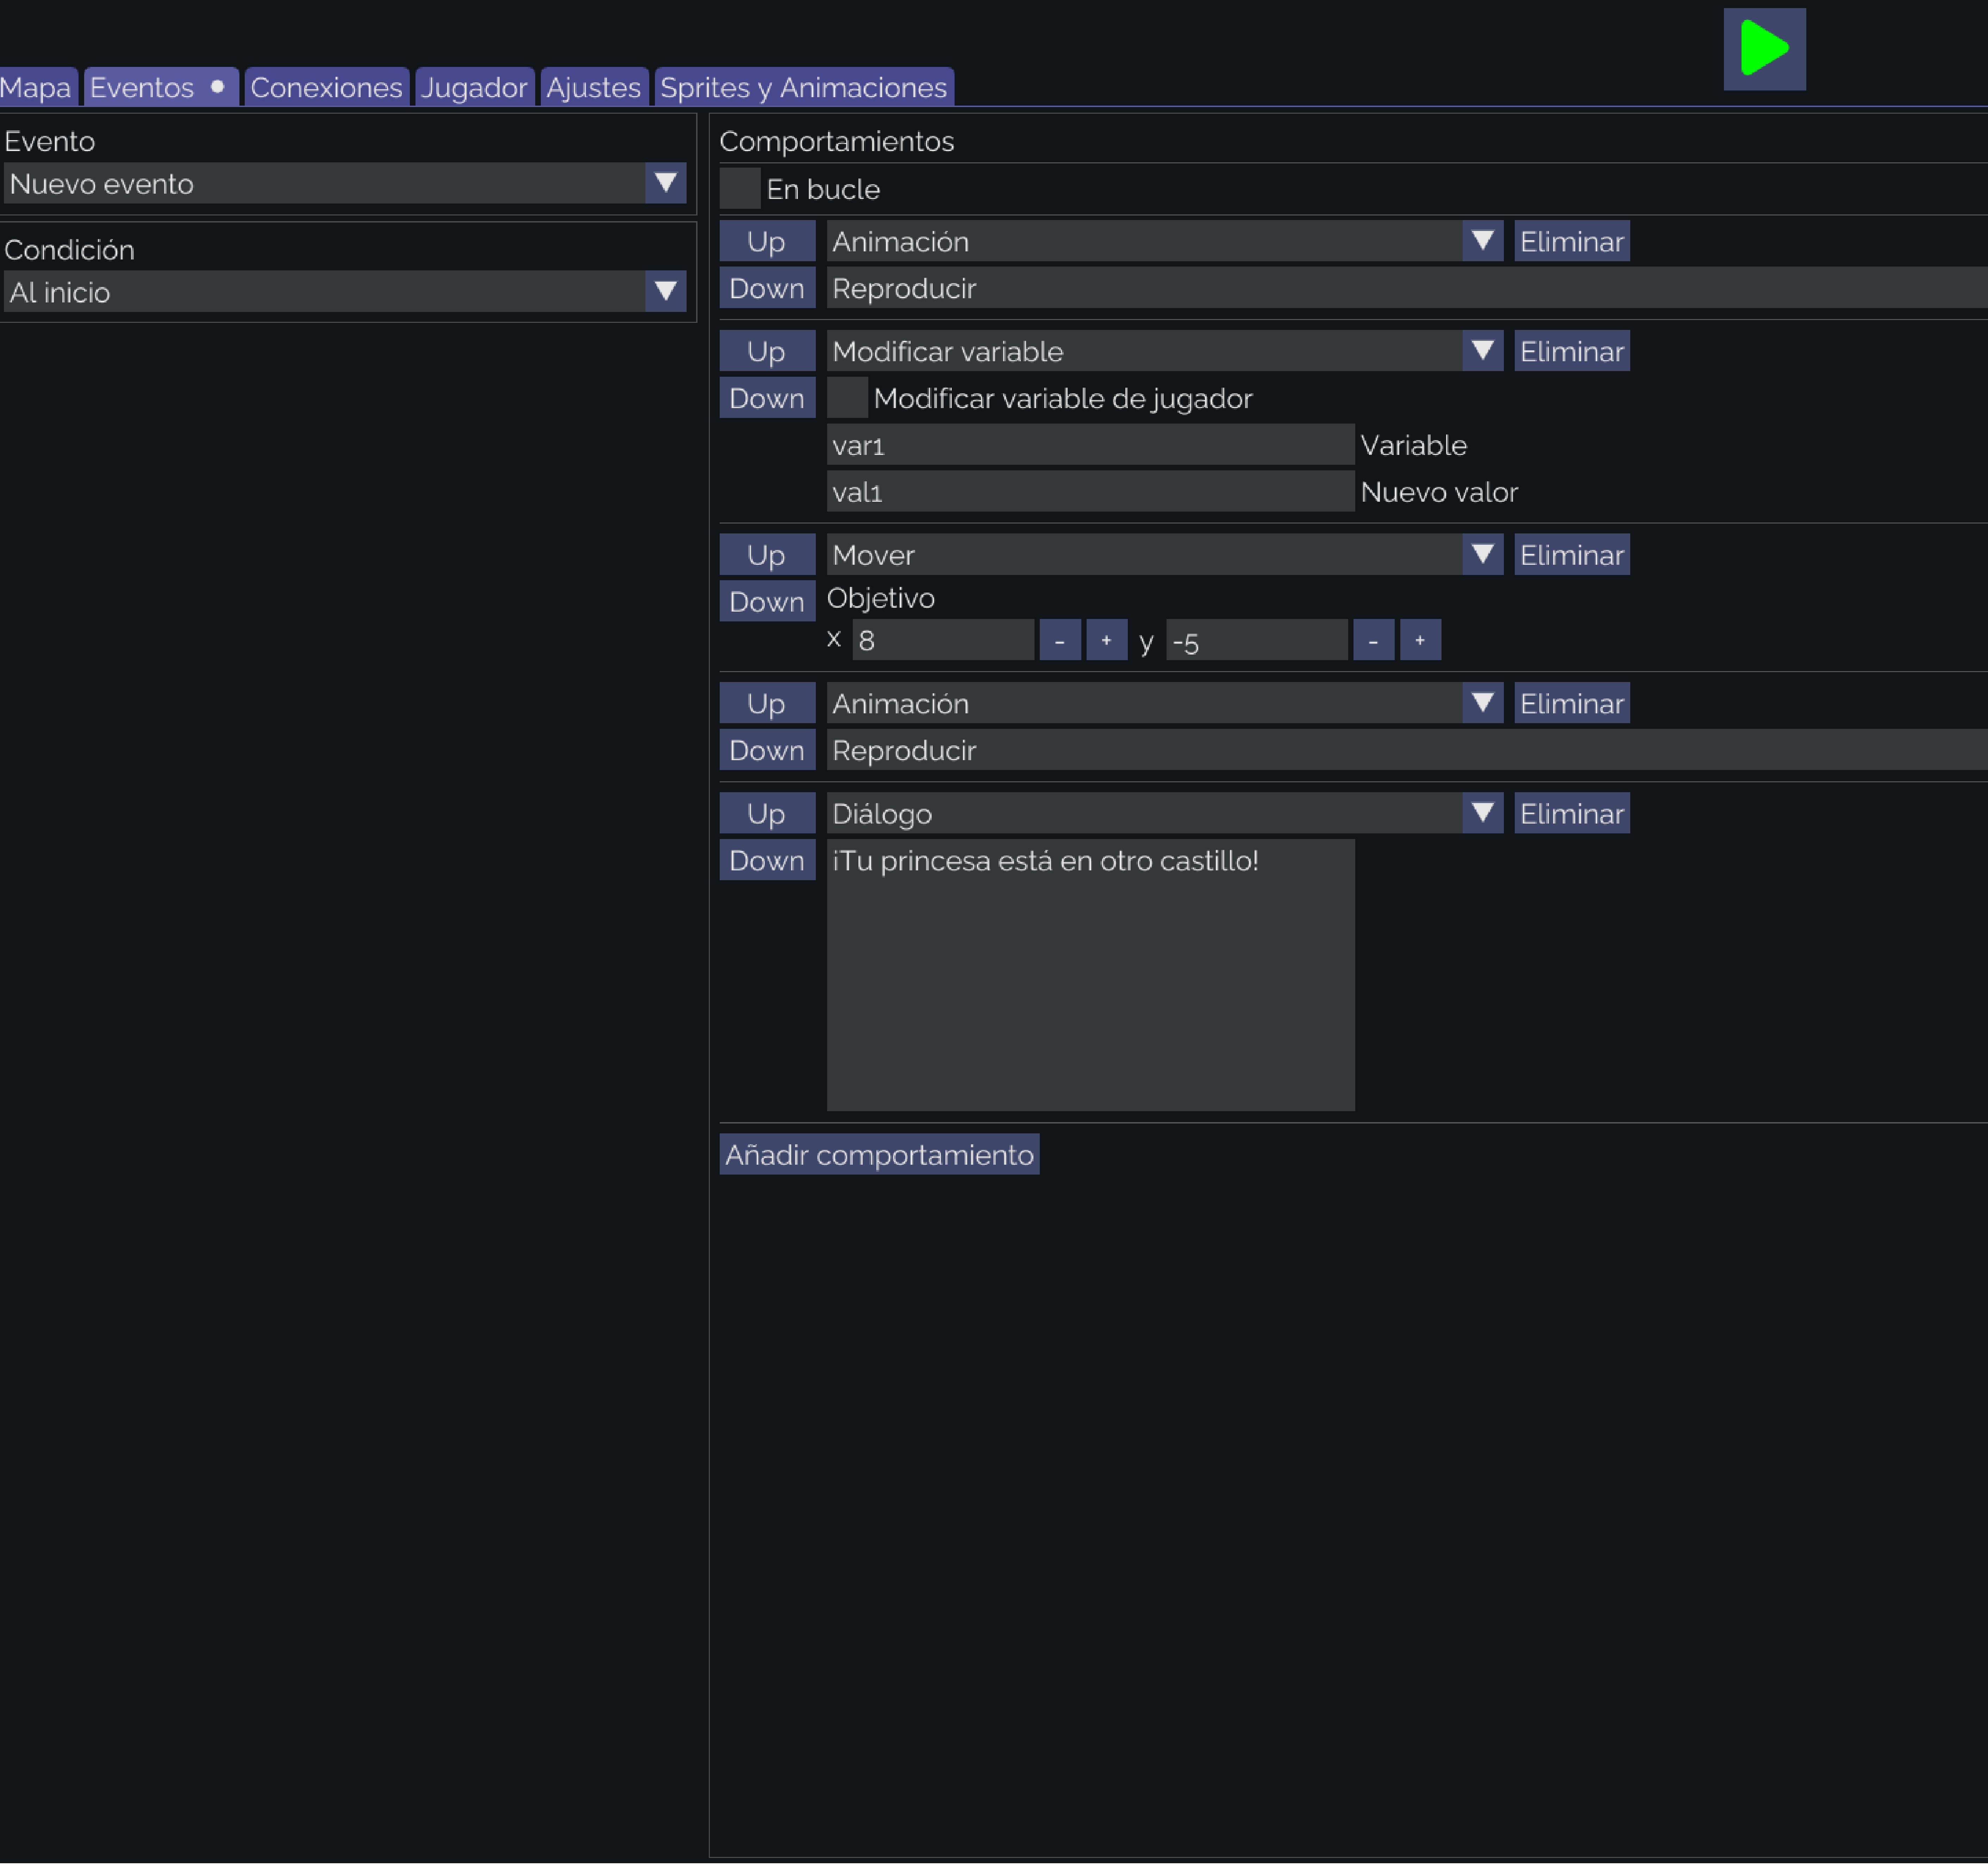
\includegraphics[width=\textwidth]{imgs/editor/eventos.pdf}
	\end{columns}
\end{frame}

\begin{frame}{\textit{Build} multiplataforma al motor}
	\begin{columns}
		 \column{0.4\textwidth}
		 	\begin{itemize}
		 		\item Se generan ejecutables para Windows, MacOS, Linux y Android.
		 		\item No requiere de recompilación manual ni de pasos adicionales.
		 		\item El editor \comillas{traduce} sus datos a la sintaxis esperada por el motor.
		 	\end{itemize}
		 \column{0.6\textwidth}
		 	\begin{center}
		 	\scalebox{0.5}{
		 	\begin{tikzpicture}[node distance=1.5cm and 2cm]
		 		\node (start) [startstop] {Usuario diseña el juego en el editor};
		 		\node (data) [process, below=of start] {Datos del proyecto};
				\node (convert) [process, below=of data] {Serialización y empaquetado};
				\node (build) [process, below=of convert] {Generación del ejecutable};
				\node (win) [io, below left=1.5cm and 2.5cm of build] {Windows};
				\node (mac) [io, below left=1.5cm and -1.0cm of build] {MacOS};
				\node (linux) [io, below right=1.5cm and -1.0cm of build] {Linux};
				\node (andr) [io, below right=1.5cm and 2.5cm of build] {Android};
				
				\draw [arrow] (start) -- (data);
				\draw [arrow] (data) -- (convert);
				\draw [arrow] (convert) -- (build);
				\draw [arrow] (build) -- (win);
				\draw [arrow] (build) -- (mac);
				\draw [arrow] (build) -- (linux);
				\draw [arrow] (build) -- (andr);
		 	\end{tikzpicture}
		 	}
		 	\end{center}
	\end{columns}
\end{frame}


\section{Pruebas con usuarios}
\begin{frame}{Objetivos de las pruebas}
		\begin{columns}
		\column{0.5\textwidth}
		\begin{itemize}
			\item ¿Entienden los usuarios cómo funcionan los sistemas?
			\item ¿Son capaces de aprovecharlos de forma creativa?
		\end{itemize}
		\column{0.5\textwidth}
		
	\end{columns}
\end{frame}
\begin{frame}{Metodología}
\begin{columns}
	\column{0.5\textwidth}
	\begin{itemize}
		\item Pruebas individuales supervisadas.
		\item Guía explicativa.
		\item Usuarios con distinto nivel.
	\end{itemize}
	\column{0.5\textwidth}
	
\end{columns}
\end{frame}
\begin{frame}{Resultados}
\begin{columns}
	\column{0.5\textwidth}
	\begin{itemize}
		\item Los sistemas se entienden.
		\item Permiten la creatividad.
		\item A pesar de esto pueden ser limitados y toscos.
	\end{itemize}
	\column{0.5\textwidth}
	
\end{columns}
\end{frame}

\section{Conclusiones}
\begin{frame}{Conclusiones}
a
\end{frame}


\title[2D video game engine and editor focused on RPG game development]{Motor y editor de videojuegos en 2D enfocado al desarrollo de juegos RPG}
\author[Miguel Curros, Alejandro González and Alejandro Massó]{Miguel Curros García\\ Alejandro González Sánchez\\ Alejandro Massó Martínez}

\section{Contributions}
\begin{frame}{Miguel Curros García}
	\begin{itemize}
		\item \baker{}'s engine design.
		\item Engine low level development.
		\item Engine gameplay development.
		\item Editor resources' persistance.
		\item Editor's events' interface
		\item Editor's events' build.
	\end{itemize}
\end{frame}

\begin{frame}{Alejandro González Sánchez}
	\begin{itemize}
		\item Technical proof of concept
		\item \baker{}'s engine design.
		\item Engine low level development.
		\item Engine gameplay development.
		\item \baker{}'s Editor's interface development.
		\item Editor's building process.
	\end{itemize}
\end{frame}

\begin{frame}{Alejandro Massó Martínez}
	\begin{itemize}
		\item Research on general and specific RPG editors.
		\item \baker{}'s editor design.
		\item Project's toolchain development.
		\item \baker{}'s editor development.
		\item Report writing.
	\end{itemize}
\end{frame}

\end{document}